We report results on three main datasets across two different experimental tasks. For the two scientific datasets, we use the Pancreatic Endocrinogenesis (PE) dataset from \citet{bastidas-ponceComprehensiveSingleCell2019} (\texttt{scvelo.datasets.pancreas()}) and the Bone Marrow (BM) dataset from \citet{settyCharacterizationCellFate2019} (\texttt{scvelo.datasets.bonemarrow()}), both distributed by ScVelo \cite{bergenScVeloGeneralizingRNA2020}. These are single-cell RNA sequencing (single-cell) datasets.

For the non-scientific dataset, we use a simulated Gulf of Mexico ocean currents data from \citet{shenMultimarginalSchrodingerBridges} and hold out every other marginal as in \citet{rohbeckMODELINGCOMPLEXSYSTEM2025, theodoropoulosMomentumMultiMarginalSchrodinger2025}.

\subsection{Pancreatic Endrocrinogensis (PE) single-cell RNA sequencing}
This dataset consists of mouse pancreatic epithelial cells at embryonic day 15.5, with ~3,696 cells and ~28k genes in the full dataset. We group clusters into 5 sequential developmental stages along the secondary endocrine transition (Ductal, Ngn3 low EP, Ngn3 high EP, Pre-endocrine, Endocrine). The results, comparing to a Linear FM baseline, are shown in Table \ref{tab:pe_log1p_eucknn} and Figure \ref{fig:pancreas_pca}. We see a consistent improvement with \ourmodel in mean $\mathrm{MMD}^2$ across the sweep of $\alpha$, with $\beta$ fixed at $0$ (pure spectral OT, no Euclidean distance term). We see the best performance at every marginal except the first intermediate marginal ($t=0.25$) when training \ourmodel with $\alpha=2$, with a 24.4\% decrease in mean $\mathrm{MMD}^2$ compared to the Linear FM baseline. These results are shown for data that is log1p encoded (normalize total counts to 10k and then pointwise $x=\log(x+1)$), when we instead perform Helligner sphere encoding (see above), we do not see improvements by using \ourmodel with spectral OT cost (see Appendix Table \ref{tab:pe_sphere}).

\begin{table*}[t]
\centering
\caption{Pancreatic endocrinogenesis, log1p HVG ambient + Euclidean kNN graph. Chained $\mathrm{MMD}^2$ at four evaluation stages, mean $\pm$ std over 5 splits $\times$ 5 init seeds.}
\label{tab:pe_log1p_eucknn}
\renewcommand{\arraystretch}{1.15}
\setlength{\tabcolsep}{4pt}
\begin{tabular}{lcccccc}
\toprule
& \multicolumn{4}{c}{MMD$^2$ at evaluation time / stage} & & \\
\cmidrule(lr){2-5}
Method & $t{=}0.25$ & $t{=}0.50$ & $t{=}0.75$ & $t{=}1.00$ & mean & $\Delta$ \\
\midrule
Linear FM
  & 0.018$\,\pm\,0.008$
  & 0.058$\,\pm\,0.011$
  & 0.063$\,\pm\,0.010$
  & \underline{0.032}$\,\pm\,0.007$
  & 0.043$\,\pm\,0.007$
  & --- \\
Random OT
  & 0.029$\,\pm\,0.007$
  & 0.066$\,\pm\,0.016$
  & 0.056$\,\pm\,0.014$
  & 0.046$\,\pm\,0.016$
  & 0.049$\,\pm\,0.010$
  & $+15.0\%$ \\
\ourmodel $\alpha=0$
  & \underline{0.009}$\,\pm\,0.006$
  & 0.054$\,\pm\,0.010$
  & 0.065$\,\pm\,0.013$
  & 0.048$\,\pm\,0.006$
  & 0.044$\,\pm\,0.006$
  & $+3.4\%$ \\
\ourmodel $\alpha=0.5$
  & 0.009$\,\pm\,0.004$
  & 0.082$\,\pm\,0.022$
  & 0.085$\,\pm\,0.017$
  & 0.108$\,\pm\,0.021$
  & 0.071$\,\pm\,0.013$
  & $+66.6\%$ \\
\ourmodel $\alpha=1$
  & 0.020$\,\pm\,0.006$
  & \underline{0.044}$\,\pm\,0.007$
  & 0.051$\,\pm\,0.005$
  & 0.042$\,\pm\,0.009$
  & 0.039$\,\pm\,0.005$
  & $-8.2\%$ \\
\ourmodel $\alpha=1.5$
  & \textbf{0.008}$\,\pm\,0.004$
  & 0.052$\,\pm\,0.006$
  & \underline{0.047}$\,\pm\,0.011$
  & 0.033$\,\pm\,0.003$
  & \underline{0.035}$\,\pm\,0.005$
  & $-17.6\%$ \\
\ourmodel $\alpha=2$
  & 0.011$\,\pm\,0.005$
  & \textbf{0.043}$\,\pm\,0.003$
  & \textbf{0.044}$\,\pm\,0.003$
  & \textbf{0.030}$\,\pm\,0.005$
  & \textbf{0.032}$\,\pm\,0.002$
  & $-24.4\%$ \\
\bottomrule
\end{tabular}
\end{table*}


\begin{figure*}[t]
\centering
\includesvg[width=\linewidth]{figures/pancreas_pca_predictions_split42}
\caption{PC1 vs PC2 of Pancreatic Endrocrinogenesis dataset predictions, sweeping $\alpha$: The leftmost panel shows the ground truth cells. Second panel shows Linear FM baseline, remaining panels show \ourmodel with spectral-cost OT at different values of $\alpha$, with $\beta=0$ fixed. Predictions are projecting using PCA fit on test cells.}
\label{fig:pancreas_pca}
\end{figure*}

\subsection{Bone Marrow single-cell RNA sequencing}
This is a Human CD34+ progenitor cells single-cell RNA sequencing dataset containing ~5,780 cells and ~14k genes. We subset to the erythroid sub-tree and drop all other lineages to form a mostly linear structure (HSC early, HSC late, Precursor, Erythroid Early, Erythroid Terminal). After filtering to the erythroid lineage, we are left with ~3,775 cells across the 5 stages. The results, comparing to a Linear FM baseline, are shown in Table \ref{tab:bm_sphere} and Figure \ref{fig:bonemarrow_pca}. For the bone marrow dataset, we show results when the data is encoded using the Hellinger sphere encoding, because we find that using spectral OT costs does not improve performance over the linear FM baseline when encoding data in log1p space (see Appendix Table \ref{tab:bm_log1p_eucknn}). Again, we see an improvement across all marginals for \ourmodel, with \ourmodel $\alpha=1$ having the best mean performance and performance on the last two marginals, while \ourmodel $\alpha=0$ has the best performance on the first two intermediate marginals ($t=0.25$ and $t=0.50$). \ourmodel $\alpha=1$ shows a 44.3\% improvement in mean $\mathrm{MMD}^2$ compared to the Linear FM baseline. For this test, we also fix $\beta=0$.

\begin{table*}[t]
\centering
\caption{Bone marrow, Hellinger sphere encoding. Chained $\mathrm{MMD}^2$ at four evaluation stages, mean $\pm$ over 5 splits $\times$ 5 init seeds.}
\label{tab:bm_sphere}
\renewcommand{\arraystretch}{1.15}
\setlength{\tabcolsep}{4pt}
\begin{tabular}{lcccccc}
\toprule
& \multicolumn{4}{c}{MMD$^2$ at evaluation time / stage} & & \\
\cmidrule(lr){2-5}
Method & $t{=}0.25$ & $t{=}0.50$ & $t{=}0.75$ & $t{=}1.00$ & mean & $\Delta$ \\
\midrule
Linear FM
  & 0.019$\,\pm\,0.003$
  & 0.151$\,\pm\,0.014$
  & 0.419$\,\pm\,0.034$
  & 0.319$\,\pm\,0.045$
  & 0.227$\,\pm\,0.022$
  & --- \\
Random OT
  & 0.017$\,\pm\,0.004$
  & 0.094$\,\pm\,0.004$
  & 0.329$\,\pm\,0.036$
  & 0.270$\,\pm\,0.053$
  & 0.177$\,\pm\,0.022$
  & $-21.9\%$ \\
\ourmodel $\alpha=0$
  & \textbf{0.015}$\,\pm\,0.005$
  & \textbf{0.058}$\,\pm\,0.011$
  & \underline{0.256}$\,\pm\,0.056$
  & \underline{0.201}$\,\pm\,0.062$
  & \underline{0.133}$\,\pm\,0.031$
  & $-41.5\%$ \\
\ourmodel $\alpha=0.5$
  & 0.017$\,\pm\,0.005$
  & 0.064$\,\pm\,0.006$
  & 0.260$\,\pm\,0.034$
  & 0.218$\,\pm\,0.046$
  & 0.140$\,\pm\,0.020$
  & $-38.4\%$ \\
\ourmodel $\alpha=1$
  & 0.017$\,\pm\,0.006$
  & \underline{0.059}$\,\pm\,0.010$
  & \textbf{0.242}$\,\pm\,0.034$
  & \textbf{0.187}$\,\pm\,0.028$
  & \textbf{0.126}$\,\pm\,0.017$
  & $-44.3\%$ \\
\ourmodel $\alpha=1.5$
  & \underline{0.016}$\,\pm\,0.005$
  & 0.077$\,\pm\,0.014$
  & 0.310$\,\pm\,0.044$
  & 0.239$\,\pm\,0.047$
  & 0.160$\,\pm\,0.026$
  & $-29.3\%$ \\
\ourmodel $\alpha=2$
  & 0.017$\,\pm\,0.006$
  & 0.082$\,\pm\,0.006$
  & 0.312$\,\pm\,0.026$
  & 0.253$\,\pm\,0.042$
  & 0.166$\,\pm\,0.017$
  & $-26.8\%$ \\
\bottomrule
\end{tabular}
\end{table*}


\begin{figure*}[t]
\centering
\includesvg[width=\linewidth]{figures/bonemarrow_pca_predictions_split42}
\caption{PC1 vs PC2 of Bone Marrow dataset predictions, sweeping $\alpha$: The leftmost panel shows the ground truth cells. Second panel shows Linear FM baseline, remaining panels show \ourmodel with spectral-cost OT at different values of $\alpha$, with $\beta=0$ fixed. Predictions are projecting using PCA fit on test cells.}
\label{fig:bonemarrow_pca}
\end{figure*}

\subsection{Gulf of Mexico Ocean Currents}
The Gulf of Mexico ocean currents dataset is built by \citet{shenMultimarginalSchrodingerBridges} and contains simulated particles that evolve based on a measured ocean current vector field. It contains 1000 particles across 9 marginals. Unlike the single-cell datasets, for this task, we follow \citet{rohbeckMODELINGCOMPLEXSYSTEM2025} and \citet{shenMultimarginalSchrodingerBridges} in using 5 marginals (odd numbers) as the training data and 4 marginals as the testing data. For the 4 held-out marginals, all 100 samples are in the test set, for the 5 training marginals, we perform an 80/10/10 train/val/test split to evaluate on unseen particles from those marginals at test-time. We perform a grid search over the $\alpha$ and $\beta$ parameters specified in \ref{sec:spec_dist_fam}, a total of 25 combinations, and compare the results of the best model to a linear FM baseline. Results are shown in Table \ref{tab:gom_otpfm9_w2}, where we report $W_2$ on each marginal and averaged over the held-out and train marginals for both models. We show that \ourmodel with $\alpha=0.5,\beta=0.0$ outperforms the linear FM baseline on every marginal, by an average of 45.5\% on the held-out marginals and $54.1\%$ on the train marginals.

\begin{figure*}[t]
\centering
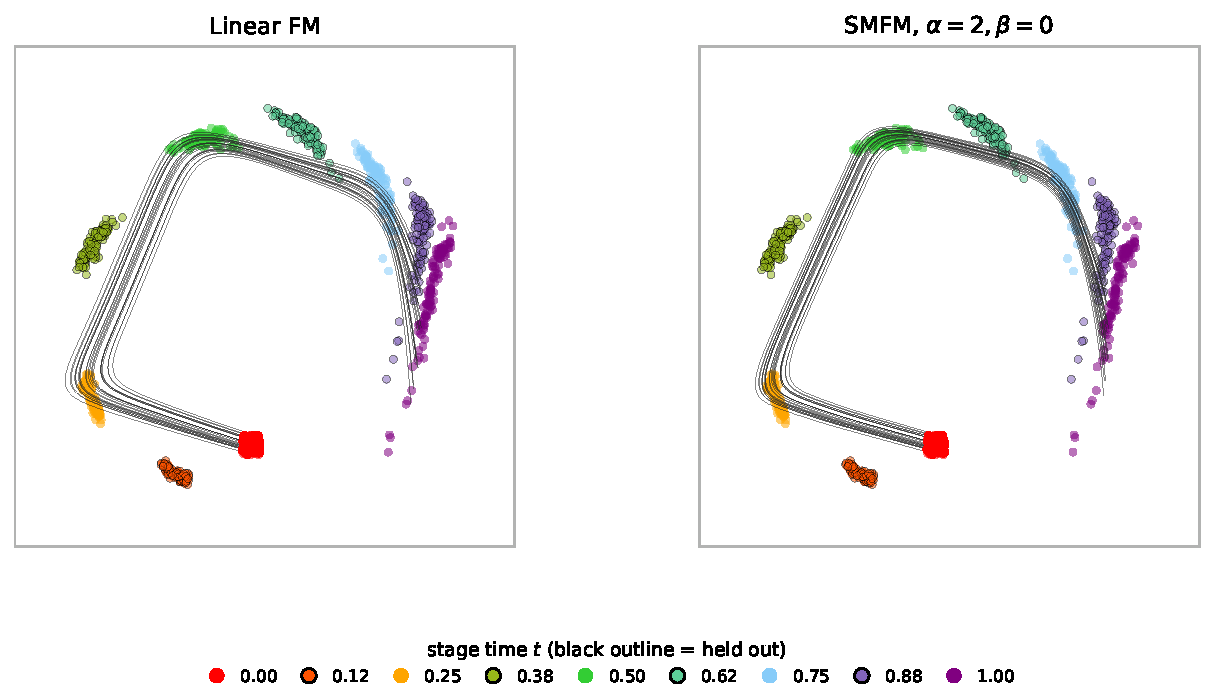
\includegraphics[width=0.7\linewidth]{figures/gom_trajectories.pdf}
\caption{GoM trajectories: Visualization of predicted trajectories on Gulf of Mexico simulated dataset. Left panel shows Linear FM with Euclidean optimal transport cost, right panel shows best \ourmodel sweeping $\alpha$ with $\beta=0$ fixed. Held-out marginals are shown with black outlines on the point. First marginal is red, last marginal is purple. The trajectories shown in both panels are predicted, all the points shown are the ground truth marginals.}
\label{fig:gom_trajectories}
\end{figure*}
\begin{table*}[t]
\centering
\caption{Per-stage chained $W_2$ on the Gulf of Mexico (GoM) 9-stage protocol with held-out marginals $\{1,3,5,7\}$. \ourmodel uses $\alpha=0.5$, $\beta=0$ with the Euclidean-cost kNN graph. Linear FM is the multi-marginal Euclidean baseline. Cells are mean$\,\pm\,$std over 5 splits $\times$ 5 init seeds.}
\label{tab:gom_otpfm9_w2}
\renewcommand{\arraystretch}{1.15}
\setlength{\tabcolsep}{6pt}
\begin{tabular}{lcccccc}
\toprule
Stage & $t$ & role & MM+Linear $W_2$ & \ourmodel $W_2$ & $\Delta\%$ \\
\midrule
$s_{1}$ & $0.12$ & held & $0.433\pm0.006$ & $0.429\pm0.004$ & $-0.9\%$  \\
$s_{2}$ & $0.25$ & train & $0.144\pm0.021$ & \textbf{$0.121\pm0.023$} & $-16.3\%$ \\
$s_{3}$ & $0.38$ & held & $0.825\pm0.019$ & \textbf{$0.477\pm0.033$} & $-42.1\%$  \\
$s_{4}$ & $0.50$ & train & $0.918\pm0.034$ & \textbf{$0.317\pm0.041$} & $-65.5\%$  \\
$s_{5}$ & $0.62$ & held & $0.989\pm0.031$ & \textbf{$0.401\pm0.053$} & $-59.4\%$  \\
$s_{6}$ & $0.75$ & train & $1.065\pm0.043$ & \textbf{$0.454\pm0.065$} & $-57.4\%$  \\
$s_{7}$ & $0.88$ & held & $1.176\pm0.067$ & \textbf{$0.556\pm0.068$} & $-52.7\%$  \\
$s_{8}$ & $1.00$ & train & $1.264\pm0.089$ & \textbf{$0.666\pm0.088$} & $-47.3\%$  \\
\midrule
\multicolumn{3}{l}{\emph{avg.\ over held-out marginals (1,3,5,7)}} & $0.856\pm0.026$ & \textbf{$0.466\pm0.036$} & $-45.5\%$  \\
\multicolumn{3}{l}{\emph{avg.\ over train marginals (0,2,4,6,8)}} & $0.848\pm0.035$ & \textbf{$0.390\pm0.043$} & $-54.1\%$  \\
\bottomrule
\end{tabular}
\end{table*}
